\documentclass[10pt,a4paper]{article}
\usepackage[utf8]{inputenc}
\usepackage[T1]{fontenc}
\usepackage{lmodern}
\usepackage[margin=1.9cm,top=2.2cm,bottom=2cm]{geometry}
\usepackage{booktabs,tabularx,array,enumitem,fancyhdr,titlesec,xcolor,microtype}
\usepackage{pgfplots}
\pgfplotsset{compat=1.16}
\usepackage[hidelinks]{hyperref}

% Replace with the public repository of the team before submitting.
\newcommand{\repourl}{https://github.com/OscarSantiagoMerino/DataForge-Consulting}

\definecolor{forge}{HTML}{0B4F71}
\definecolor{teal}{HTML}{12908E}
\definecolor{alert}{HTML}{B5123B}

\pagestyle{fancy}\fancyhf{}
\lhead{\small Sprint Report, Second Term. FinBank S.A.}
\rhead{\small DataForge Consulting}
\cfoot{\small\thepage}
\titleformat{\section}{\normalsize\bfseries\color{forge}}{\thesection.}{0.5em}{}
\titlespacing*{\section}{0pt}{9pt}{4pt}
\setlength{\parindent}{0pt}\setlength{\parskip}{4pt}
\setlist{nosep,leftmargin=1.2em}
\newcolumntype{L}{>{\raggedright\arraybackslash}X}
\renewcommand{\arraystretch}{1.12}

\begin{document}

\begin{center}
{\Large\bfseries Sprint Report and Agile Metrics}\\[2pt]
Predictive Analytics Program: Sprints 1 and 2 executed with Scrum and XP\\[2pt]
{\small Client: FinBank S.A., Vice Presidency of Risk and Analytics \quad Project code: GMAC-FB-2026-01}\\
{\small Daniel Felipe Martínez Hernández \,·\, Rafael Alejandro Baracaldo Doikov \,·\, Oscar Santiago Merino Suárez}
\end{center}
\vspace{-6pt}\rule{\linewidth}{0.4pt}

\section{What this report covers}
In the first term the same two sprints were run with PMBOK for control and a Kanban board for delivery,
and were reported through flow metrics. This report runs the same simulated engagement again, with the same backlog,
the same 12 weeks and COP \$180,000,000 fixed by the Charter, and the same impediment, but managed with
\textbf{Scrum} (events, commitment, velocity) and \textbf{Extreme Programming} (pairing, test-first rules, continuous
integration, simple design). Section 7 states what changed in the way of working. Scrum accountabilities:
Rafael Baracaldo, Product Owner; Oscar Merino, Scrum Master; the three members are Developers, and Daniel
Martínez keeps the formal reporting to the sponsor required by the Charter.

\section{Sprint closure}
{\small
\begin{tabularx}{\linewidth}{@{}l l L c c l@{}}
\toprule
Sprint & Dates (2026) & Sprint Goal & Committed & Done & Goal \\
\midrule
S1 & 10--21 Aug & The engagement is governed and the team can touch data legally. & 16 & 16 & Met \\
S2 & 24 Aug--4 Sep & A validated data foundation for the delinquency and churn models. & 20 & 15 & Partly met \\
\bottomrule
\end{tabularx}

\vspace{5pt}
\begin{tabularx}{\linewidth}{@{}l L c l@{\hspace{14pt}}l L c l@{}}
\toprule
\multicolumn{4}{@{}l}{\textbf{Sprint 1 backlog}} & \multicolumn{4}{l}{\textbf{Sprint 2 backlog}}\\
ID & Item & Pts & State & ID & Item & Pts & State \\
\midrule
US-01 & Charter approved by the sponsor & 3 & Done & T-05.0 & Extraction script, delinquency data & 2 & Done \\
US-02 & Data access agreement, Ley 1581 & 5 & Done & T-05.6 & Validation rules, written test-first & 3 & Done \\
US-03 & Client base profiling on the anonymized sample & 5 & Done & T-05.1 & Data quality report & 4 & Done \\
US-04 & Board, repository and Definition of Done & 3 & Done & T-05.4 & Delinquency target at 30 and 60 days & 3 & Done \\
 & & & & T-05.2 & Feature dictionary v1, validated by business & 3 & Done \\
 & & & & T-05.5 & Churn history extract & 5 & \textcolor{alert}{Blocked} \\
\bottomrule
\end{tabularx}}

Increment at the end of Sprint 2: a pipeline that validates an extract, produces the quality report, excludes
4 of 22 candidate variables for completeness below 80\%, documents the 18 that remain in the feature dictionary and
builds both delinquency targets. It runs with one command from the repository and is covered by 16 automated tests.
Milestone M2 is not closed, because the dictionary has no churn variables yet.

\section{Velocity and burndown}
\begin{center}
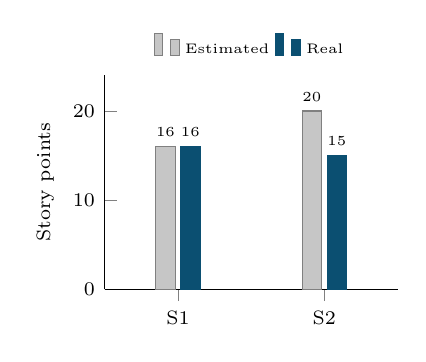
\begin{tikzpicture}
\begin{axis}[width=5.3cm,height=4.3cm,ybar,bar width=7pt,ymin=0,ymax=24,
  symbolic x coords={S1,S2},xtick=data,enlarge x limits=0.5,
  ylabel={Story points},ylabel style={font=\scriptsize},tick label style={font=\scriptsize},
  nodes near coords,nodes near coords style={font=\tiny},
  legend style={font=\tiny,at={(0.5,1.03)},anchor=south,legend columns=2,draw=none},
  title={},axis lines*=left]
\addplot[fill=gray!45,draw=gray] coordinates {(S1,16) (S2,20)};
\addplot[fill=forge,draw=forge] coordinates {(S1,16) (S2,15)};
\legend{Estimated,Real}
\end{axis}
\end{tikzpicture}\hfill
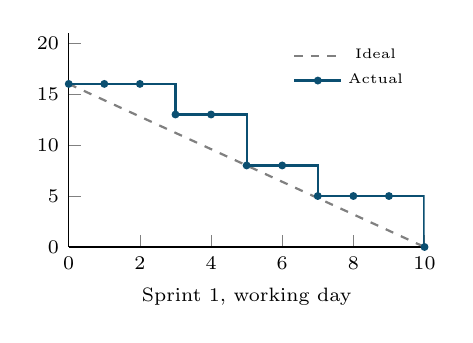
\begin{tikzpicture}
\begin{axis}[width=6.1cm,height=4.3cm,xmin=0,xmax=10,ymin=0,ymax=21,xtick={0,2,...,10},
  xlabel={Sprint 1, working day},label style={font=\scriptsize},tick label style={font=\scriptsize},
  legend style={font=\tiny,draw=none,at={(0.98,0.98)},anchor=north east},axis lines*=left]
\addplot[dashed,gray,thick] coordinates {(0,16) (10,0)};
\addplot[const plot,forge,thick,mark=*,mark size=1pt] coordinates
 {(0,16) (1,16) (2,16) (3,13) (4,13) (5,8) (6,8) (7,5) (8,5) (9,5) (10,0)};
\legend{Ideal,Actual}
\end{axis}
\end{tikzpicture}\hfill
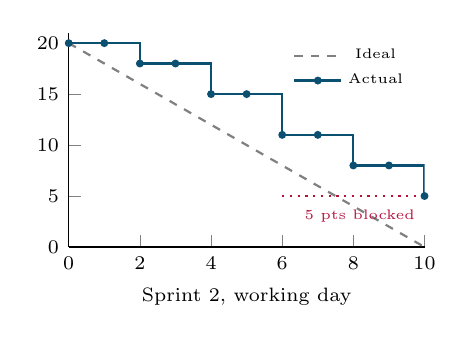
\begin{tikzpicture}
\begin{axis}[width=6.1cm,height=4.3cm,xmin=0,xmax=10,ymin=0,ymax=21,xtick={0,2,...,10},
  xlabel={Sprint 2, working day},label style={font=\scriptsize},tick label style={font=\scriptsize},
  legend style={font=\tiny,draw=none,at={(0.98,0.98)},anchor=north east},axis lines*=left]
\addplot[dashed,gray,thick] coordinates {(0,20) (10,0)};
\addplot[const plot,forge,thick,mark=*,mark size=1pt] coordinates
 {(0,20) (1,20) (2,18) (3,18) (4,15) (5,15) (6,11) (7,11) (8,8) (9,8) (10,5)};
\addplot[alert,thick,dotted] coordinates {(6,5) (10,5)};
\node[font=\tiny,text=alert,anchor=north east] at (axis cs:10,4.6) {5 pts blocked};
\legend{Ideal,Actual}
\end{axis}
\end{tikzpicture}
\end{center}
\vspace{-8pt}
{\small
\begin{tabularx}{\linewidth}{@{}l c c c L@{}}
\toprule
Sprint & Estimated & Real & Real / estimated & Reading \\
\midrule
S1 & 16 & 16 & 100\% & Four items closed; the last 5 points burned on day 10, when the access agreement was signed. \\
S2 & 20 & 15 & 75\% & The team took 4 points more than it had just proved it could deliver, and 5 points depended on a credential owned by IT. \\
\midrule
Average velocity & & 15.5 & & Capacity used to plan Sprint 3. \\
\bottomrule
\end{tabularx}}

The Sprint 2 curve is the one shown in the first term, and it stays above the ideal line from day 2. The shortfall is
not a slower team: the 15 points that depended only on the team were all delivered, which is the Sprint 1 pace.
The 5 remaining points are a single item that could not start. The lesson is about commitment, not effort.

\section{Daily Scrum log}
Fifteen minutes at 8:00, three questions per person. The entries below are the days on which the plan changed.

{\footnotesize
\begin{tabularx}{\linewidth}{@{}l L L L@{}}
\toprule
Day & Done since the last Daily & Plan for the day & Impediments \\
\midrule
S1 D1 & Sprint Planning: 4 items, 16 points. & Daniel drafts the Charter; Oscar sets up the board; Rafael requests the anonymized sample. & None. \\
S1 D3 & Board and first Definition of Done in use (US-04). Sample received. & Rafael profiles the sample; Daniel sends the agreement to the data protection officer. & Warehouse access not yet authorized (R1), covered by the sample. \\
S1 D5 & Profiling of the client base closed (US-03). & Charter review with the sponsor. & Profiling script exists only on one laptop. \\
S1 D7 & Charter signed (US-01). & Close the observations of the data protection officer. & Agreement waiting for legal signature. \\
S1 D10 & Agreement signed (US-02). Review and Retrospective held. & Sprint 2 Planning. & None. \\
\midrule
S2 D1 & Planning: 6 items, 20 points. Repository, CI and pull request rule active. & Rafael writes the extraction script; Oscar requests the churn credential from IT. & None. \\
S2 D3 & Extraction script merged (T-05.0). & Pairing 1, Rafael drives and Daniel navigates: validation rules written as failing tests first. & None. \\
S2 D5 & Validation rules merged, 7 tests green (T-05.6). & Quality report. Oscar starts refactoring R-01. & Bounds duplicated between rules and dictionary. \\
S2 D6 & Quality report in business validation. R-01 merged. & Churn extract cannot start. & \textcolor{alert}{IT credential not issued. T-05.5 blocked.} \\
S2 D7 & Scrum Master escalated to the sponsor. Product Owner reordered the Sprint Backlog. & Pairing 2, Oscar drives and Rafael navigates: target at 30 and 60 days pulled forward. & Credential pending, day 2. \\
S2 D8 & Quality report accepted (T-05.1). Targets merged (T-05.4). & Feature dictionary v1; session with collections to validate variables. & Credential pending, day 3. \\
S2 D10 & Dictionary v1 validated: 18 variables (T-05.2). & Sprint Review with the sponsor, then Retrospective. & Credential pending, day 4. T-05.5 returns to the Product Backlog. \\
\bottomrule
\end{tabularx}}

\section{Retrospective minutes}
{\footnotesize
\begin{tabularx}{\linewidth}{@{}l L L L@{}}
\toprule
 & Start & Stop & Continue \\
\midrule
S1 & Keeping every script in a shared repository with CI. Writing the data rules as tests before the analysis. Pairing on anything that encodes a business rule. &
Keeping work on personal laptops. Accepting a result because its author says it runs. &
Asking for an anonymized sample in parallel to the access request: it kept profiling moving while R1 was open. \\
S2 & Committing no more than the average velocity. Accepting an item into a sprint only if its external dependencies are already granted (Definition of Ready). Raising a blocker the same day it appears. &
Committing points that depend on another area's calendar. Copying bounds from the dictionary into the code. &
Pairing with rotation of driver. Tests before rules. Reordering the Sprint Backlog with the Product Owner instead of waiting. \\
\bottomrule
\end{tabularx}

\vspace{4pt}
\begin{tabularx}{\linewidth}{@{}l L l l@{}}
\toprule
From & Improvement action & Owner & State \\
\midrule
S1 & Repository with CI; the Definition of Done now also requires tests green and a pull request approved by a peer. & Oscar & Done, S2 day 1 \\
S1 & At least two pairing sessions per sprint, logged in the XP log. & Rafael & Done in S2 \\
S2 & Sprint 3 commitment capped at 16 points. & Rafael & Applied in section 8 \\
S2 & Definition of Ready: no item with an ungranted external dependency enters a sprint. & Oscar & For S3 Planning \\
S2 & Impediments are escalated by the Scrum Master within 24 hours. & Oscar & In force \\
\bottomrule
\end{tabularx}}

\section{XP practices}
{\footnotesize
\begin{tabularx}{\linewidth}{@{}l L L@{}}
\toprule
Practice & How it was applied & Evidence in the repository \\
\midrule
Pair programming & Two sessions in Sprint 2 with driver and navigator, rotating the driver. & Co-authored commits; \texttt{docs/XP\_LOG.md}, practice 01. \\
Test-driven development & Rules for ranges, categories, identifiers and personal data written as failing tests before the code. & 16 tests in \texttt{tests/}; execution report in the CI run of each pull request. \\
Continuous integration, collective ownership & One branch per item, pull request approved by a member who did not write it, tests run on every push. & Pull request history on \texttt{main}; \texttt{.github/workflows/ci.yml}. \\
Simple design, refactoring & R-01: validation rules now read their bounds from the dictionary schema. From 99 lines covering 5 variables to 84 lines covering 22. & \texttt{docs/refactoring/}; \texttt{docs/XP\_LOG.md}, practice 04. \\
\bottomrule
\end{tabularx}}

Repository: \url{\repourl}

\section{Differences in the workflow: first term and second term}
The Charter did not change, and neither did the backlog or the impediment. What changed is what the team
commits to, what it measures and what it accepts as finished.

{\footnotesize
\begin{tabularx}{\linewidth}{@{}>{\raggedright\arraybackslash}p{2.5cm} L L@{}}
\toprule
 & First term: PMBOK and Kanban & Second term: Scrum and XP \\
\midrule
Unit of work & The card. Work is pulled when a column has room under its WIP limit. The sprint is a funding gate. & The sprint. Planning fixes a Sprint Goal and a number of points the team commits to. \\
Roles & Project Leader, Business Analyst and Scrum Facilitator, with a RACI and one owner per card. & Product Owner, Scrum Master and Developers. Any member can change any file. \\
Metrics & Throughput, cycle time of 3.2 days, WIP compliance, cost and schedule variance. & Velocity, estimated against real, and burndown. \\
Question the metrics answer & Where is work stuck, and are we inside the baseline? & How much can we promise for the next sprint? \\
Impediment & Card moved to Blocked on day 6. Escalated on day 7 through change control, because it exceeded the mitigation of R1. & Raised at the Daily Scrum on day 6. The Scrum Master escalates and the Product Owner reorders the sprint the next morning. \\
Finished means & Reproducible, documented, validated by the business owner and shown in a review. & The same, plus tests green in CI and a pull request approved by a peer. \\
Quality control & Review by the business owner at the end, in the Client Validation column. & Built in before the business sees it: tests first, pairing, peer review. \\
Improvement & The sponsor decides at the gate: continue, redirect or stop. & The gate remains. The team adds its own Retrospective with owned actions. \\
Review with client & Status of variance, risks and board. & The same figures, after a live demonstration of the increment. \\
\bottomrule
\end{tabularx}}

Three consequences were visible in the simulation. First, Kanban showed \emph{that} a card was stuck, while velocity showed
that Sprint 2 had been over-committed from its first day, which the flow metrics could not say. Second, the
Definition of Done became stricter, and the same 15 points now carry tests and a second reader, so no part of the pipeline
depends on one person. Third, Scrum gave the team less freedom inside the sprint: Kanban let it pull the next card at any
moment, while here every reordering went through the Product Owner. The PMBOK layer was not replaced. The Charter, the
reserve and change control still frame every sprint.

\section{Forecast for Sprint 3}
With an average velocity of 15.5, Sprint 3 is planned at 16 points at most: the delinquency model (US-06, 13 points) is
the Sprint Goal and protects objective O1 in week 6. The churn extract (5 points) enters only if the credential exists
at Planning. The weekly early warning list (US-07, 5 points) moves to Sprint 4, which would then hold 23 points against
a capacity of 16. Milestone M4 in week 8 is therefore at risk, and this is the decision brought to the sponsor at the
Sprint Review.

\end{document}
